\sisetup{separate-uncertainty=true}
\sisetup{multi-part-units=single}
\section{Methods and results}
\label{Method}
% The setup of the experiment and preanalysis are discussed in Section~\ref{sec:laserstage}. Analysis method and results of parameters are introduced in the following sections.
\subsection{Preanalysis}
\label{sec:laserstage}

The laser intensity is adjusted to the level of $1/20$ occupancy to obtain single PE events. The window size $T_{\mathrm{wave}}$ is \SI{10400}{ns} to include all the possible after-pulses (see Section~\ref{sec:afterpulse}). The rising edge of the trigger waveform from the laser system is linearly interpolated to get the half-height time $t_{\mathrm{trig}}$ at about \SI{250}{ns}, as shown in Fig.~\ref{fig:triggertime}.
\begin{figure}[!htbp]
    \centering
    \includegraphics[width=\LF\textwidth]{figures/method/triggerwave.pdf}
    \caption{An example of PMT and trigger signals. The orange line is the trigger waveform in arbitrary scale. The green cross is the interpolated trigger time $t_{\mathrm{trig}}$. The solid blue line is the PMT waveform with a PE pulse. The horizontal violet dotted line is the voltage threshold for calculating the baseline shown by the blue horizontal dashed line. The black horizontal dash lines intersect 10\%, 50\% and 90\% of (downward) rising and falling edges. The rise and fall times are the interval lengths between 10\% and 90\% of the respective edges. The red and yellow vertical dashed lines are for the 10\% rising edge and the pulse peak.}
    \label{fig:triggertime}
\end{figure}


In the preanalysis, we select a preliminary window $[t_{\mathrm{trig}},600\,\mathrm{ns}]$ where dark noises (\SI{< 10}{kHz} in Section~\ref{sec:dcr}) and laser pulses are expected to contribute 0.004 and 0.05 counts on average. The peak time $t_p$ is the minimum position in each window, as shown in Fig.~\ref{fig:triggertime}.
%Because the maximum pulse is selected in each waveform, the expected charge distribution is the distribution of $\max(C_n)$ ($n=1,...,N$), in which $C_n$ is the charge of the nth PE and $N$ is the number of PE in a waveform.


The nonzero baseline is estimated from the sidebands $[-200\,\mathrm{ns},-10\,\mathrm{ns}]$ and $[100\,\mathrm{ns},200\,\mathrm{ns}]$ relative to $t_p$. % padding
To remove potential additional pulses in the sidebands, we define a voltage threshold from a rough estimation of white noise as the horizontal violet dotted line in Fig.~\ref{fig:triggertime} and cut off additional \SI{10}{ns} around each over-threshold time interval. The baseline $\mu_b$ is estimated as the average of the residual sidebands. The peak height $V_p$ of a pulse is the difference between $\mu_b$ and the minimum voltage at \(t_p\).

Over all the waveform samples, a Gaussian $f(t;t_0,\sigma_{t0}^2)$ is fitted to the distribution of $t_p-t_{\mathrm{trig}}$ of pulses whose $V_p$ exceeds \SI{5}{ADC}. We define a new candidate window, about \SI{30}{ns} long, as $[t_0-5\sigma_{t0}, t_0+5\sigma_{t0}]$ to calculate new $t_p$ and $V_p$ by repeating the above procedures.  The contracted time window reduces the dark counts by 10 times, with which we shall conduct the charge and time characterization of the single PE in the following sections.

\subsection{Single-PE charge spectrum and resolution}
\label{sec:noisepeak}

Considering the rise and fall time distributions, the charge $Q$ of a pulse is defined as % padding
the summation of the baseline-subtracted voltages in a time window $[\SI{-10}{ns}, \SI{75}{ns}]$ relative to $t_p$ as illustrated in the pink region of Fig.~\ref{fig:triggertime}. The input impedance being \SI{50}{\Omega}~\cite{CAENV1751}, the charge in Coulomb is $Q/\SI{50}{\Omega}$.

Such $Q$ in Fig.~\ref{fig:triggercharge} represents the charge of a single PE with negligible multi-PE contributions due to the low occupancy. A long tail is evident in the single-PE charge distribution, which was also found in the NNVT 20-inch MCP-PMTs by the JUNO collaboration~\cite{JUNOMassTesting}. Zhang~et~al.~\cite{JUNOLongtail} proposed a phenomenological parameterization without dedicated consideration of the multiplication process of the PEs. We shall discuss the physical model and solution of the long tail in our future publications.

To describe the peak shape of the $Q$ distribution, a Gaussian function $N^{\mathrm{1e}}f(Q;Q_0,\sigma^2_{Q_0})$ is fitted to the interval $[0.65Q_0, 1.35Q_0]$ via the modified least-square (MLS)~\cite{Cowan1998StatisticalDA} illustrated as the red line in Fig.~\ref{fig:triggercharge}. To remove the influence of the pedestal and describe the long tail, $N^{\mathrm{hit}}$ pulses with $V_p>\SI{3}{ADC}$ and $Q>0.25Q_0$ are selected to calculate the mean $\overline{Q}$ and sample variance $s^2_{Q}$ of $Q$. The Gaussian component ratio $N^{\mathrm{1e}}/N^{\mathrm{hit}}$ ($0.59\pm0.02$ for the nine MCP-PMTs) of charge distribution reflects the significance of long tail.

\begin{figure}[!htbp]
    \centering
    \begin{subfigure}[b]{\SF\textwidth}
        \includegraphics[width=\textwidth]{figures/method/triggercharge.pdf}
        \caption{}%PM
        \label{fig:triggercharge}
    \end{subfigure}
    \begin{subfigure}[b]{\SF\textwidth}
        % \includegraphics[width=\textwidth]{figures/method/triggerpeak.pdf}
        % \caption{}%PM
        % \label{fig:triggerpeak}
        \includegraphics[width=\textwidth]{figures/result/gainres.pdf}
        \caption{}
        \label{fig:totalchargeCompare}
    \end{subfigure}
    \caption{(\subref{fig:triggercharge}) The long-tailed single-PE charge distribution of an MCP-PMT. The entries around zero are waveforms with no signal. The vertical blue dashed line is the pedestal cut. The orange histogram is the selected waveforms with peak-height cut ($V_p>\SI{3}{ADC}$). The pink and green areas are the fit intervals for the peak and valley parameters. A Gaussian function $f(Q;Q_0,\sigma^2_{Q_0})$ is fitted to the peak of single-PE charge distribution. Mean $\overline{Q}$ and sample variance $s_Q^2$ of selected charge reflect the long-tailed information. (\subref{fig:totalchargeCompare}) The charge and resolution ratios show the effect of the long tail. The point and crosses represent the reference and MCP-PMTs, respectively.
    }
\end{figure}

The gains of the main peak and the entire sample are ${Q_0}/({\SI{50}{\Omega}} e) \approx \num{e7}$ and ${\overline{Q}}/(\SI{50}{\Omega} e)$, $e$ being the charge of an electron. The relative \emph{peak} and \emph{sample resolutions} $\nu_0$ and $\nu$ are defined as ${\sigma_{Q_0}}/{Q_0}$ and \(\left.{\sqrt{s^2_{Q}}}\middle/{\overline{Q}}\right.\). Fig.~\ref{fig:totalchargeCompare} indicates that $\overline{Q}$ is about 1.8 times $Q_0$ for the MCP-PMTs, in agreement with Zhang~et~al.~\cite{JUNOLongtail}. The long tail causes the resolution of MCP-PMTs to degrade from $\nu_0=\num{0.25 \pm 0.02}$ to $\nu=\num{0.69 \pm 0.03}$, which is less pronounced for the reference dynode PMT.

\subsection{Peak-to-valley ratio}
\label{sec:PV}
A parabolic function is fitted to the valley based on MLS in the interval $[-0.15Q_0, 0.25Q_0]$ relative to the least-counted bin of the histogram between the pedestal and the main peak, as shown in Fig.~\ref{fig:triggercharge}. The \emph{valley count} $N_v$ is defined as the minimum of the parabola and \emph{peak count} $N_p$ is the maximum of the Gaussian described in Section~\ref{sec:noisepeak}. The peak-to-valley ratio~(P/V) ${N_p}/{N_v}$ shows the ability to discriminate between electronic noises and a PE signal. The average P/V of MCP-PMTs is about 5.9, significantly higher than that (about 2.4) of the reference PMT.

\subsection{Single electron response}
\label{sec:SER}
We define $t^{10}_r$, $t^{50}_r$, $t^{90}_r$ ($t^{10}_f$, $t^{50}_f$, $t^{90}_f$) as the times of interpolated 10\%, 50\%, and 90\% $V_p$ in the rising (falling) edge as shown in Fig.~\ref{fig:triggertime}.  The rise time $t_r = t^{90}_r - t^{10}_r$, fall time $t_f = t^{10}_f - t^{90}_f$ and full width at half maximum $\mathrm{FWHM} = t^{50}_f - t^{50}_r$ describe the shape of \emph{single electron response}~(SER).  They are measured to be $t_r = \SI{3.72\pm0.15}{ns}$, $t_f = \SI{15.6\pm1.8}{ns}$ and $\mathrm{FWHM} = \SI{9.07\pm0.63}{ns}$ for the nine MCP-PMTs.

% \begin{figure}
%     \centering
%         \includegraphics[width=\MF\textwidth]{figures/method/triggerSER.pdf}
%         \caption{A fitting result of a pulse.}%PM
%         \label{fig:triggerser}
    % \begin{subfigure}[b]{\SF\textwidth}
    %     \includegraphics[width=\textwidth]{figures/result/tausigma.pdf}
    %     \caption{}%PM
    %     \label{fig:sigmaCompare}
    % \end{subfigure}
    % \caption{(a)  (b) $\tau$ versus $\sigma$ of 9 MCP-PMTs.}
% \end{figure}
To get a smooth SER, signals with $V_p>\SI{3}{ADC}$, $Q \in [0.5Q_0, \SI{1000}{\mathrm{ADC\cdot ns}}]$ and $\mathrm{FWHM} \in [2\,\mathrm{ns}, 15\,\mathrm{ns}]$ are selected to exclude the noise and large pulses. %padding
An \emph{exGaussian} distribution $f^N(t;\mu_{\mathrm{SER}},\sigma_\mathrm{SER}^2)\otimes f^{\mathrm{Exp}}(t;1/\tau_\mathrm{SER})$~\cite{Luo:2022xrd} is used to fit the SER% as shown in Fig.~\ref{fig:triggerser}
, in which $\mu_{\mathrm{SER}}$ is the pulse location, $\sigma_{\mathrm{SER}}$ and $\tau_{\mathrm{SER}}$ model its shape. They are measured to be $\tau_{\mathrm{SER}} = \SI{7.2\pm1.1}{ns}$ and $\sigma_{\mathrm{SER}} = \SI{1.62\pm0.06}{ns}$ for the nine MCP-PMTs.

\subsection{Transit time spread}
\label{sec:TTS}
As shown in Fig.~\ref{fig:mcpelectron}, the PEs from the photocathode drift to the MCP. Using a model of a cathode at \SI{0}{V}, a focusing electrode at \SI{480}{V} and an MCP at \SI{528}{V} to simulate the electric field and the PE trajectory, we find the PEs from the top of the photocathode with \SI{0}{eV} and \SI{3}{eV} kinetic energies have drift times of about \SI{21}{ns} and \SI{18}{ns} respectively. A PE entering an MCP channel is multiplied to be an observable pulse, while that hitting the surface of the MCP gets scattered inelastically into several secondary electrons or elastically into one single electron~\cite{Furman}. The scattered electrons drift in the electric field until finally entering the MCP channels to give delayed pulses~\cite{KM3NetTesting}. Multiple secondary electrons with different kinetic energies may cause two or more pulses with different drift times, one example shown in Fig.~\ref{fig:triggerTT2pulse}.

\begin{figure}[!htbp]
    \centering
    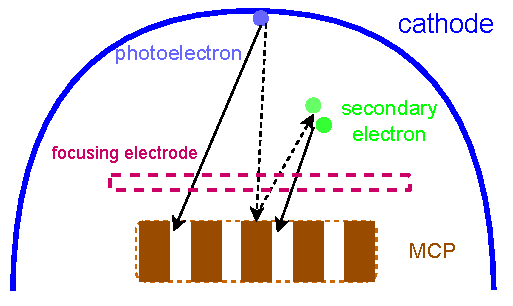
\includegraphics[width=\MF\textwidth]{figures/method/MCPelectron.pdf}
    \caption{The PEs drift from the photocathode to the MCP and get amplified or scattered.}%PM
    \label{fig:mcpelectron}
\end{figure}

The time of a PE traveling from the photocathode to the anode is called the \emph{transit time}~(TT). However, the absolute TT is hard to measure. As a convention practically, we refer to the time difference between the trigger signal $t_{\mathrm{trig}}$ and 10\% of the rise time of a PE pulse $t_r^{10}$ as TT instead. The $\mathrm{TT}$ distribution of the MCP-PMTs contains slowly rising and falling edges on both sides of the peak, as shown in Fig.~\ref{fig:triggerTTSLog}. The rising edge is due to the PEs with larger kinetic energies, while the falling one consists of secondary electrons with longer drift times~\cite{longtail}.

Delayed pulses are searched in the interval $[t_0+20\,\mathrm{ns},t_0+80\,\mathrm{ns}]$ to separate them from the main pulses in $[t_0-5\,\mathrm{ns},t_0+5\,\mathrm{ns}]$. The blue histogram in Fig.~\ref{fig:triggerTTlatepulse} is the distribution of the delayed pulses, and the filled one is for those with the main pulses in the same waveform, an example demonstrated in Fig.~\ref{fig:triggerTT2pulse}. The sharp difference between them at about \SI{40}{ns} after the main peak, twice the drift time of PEs from the cathode to the MCP, reasonably illustrates that an elastically scattered electron cannot appear together with a main pulse in a waveform.

\begin{figure}[!htbp]
    \centering
    \begin{subfigure}[t]{\SF\textwidth}
        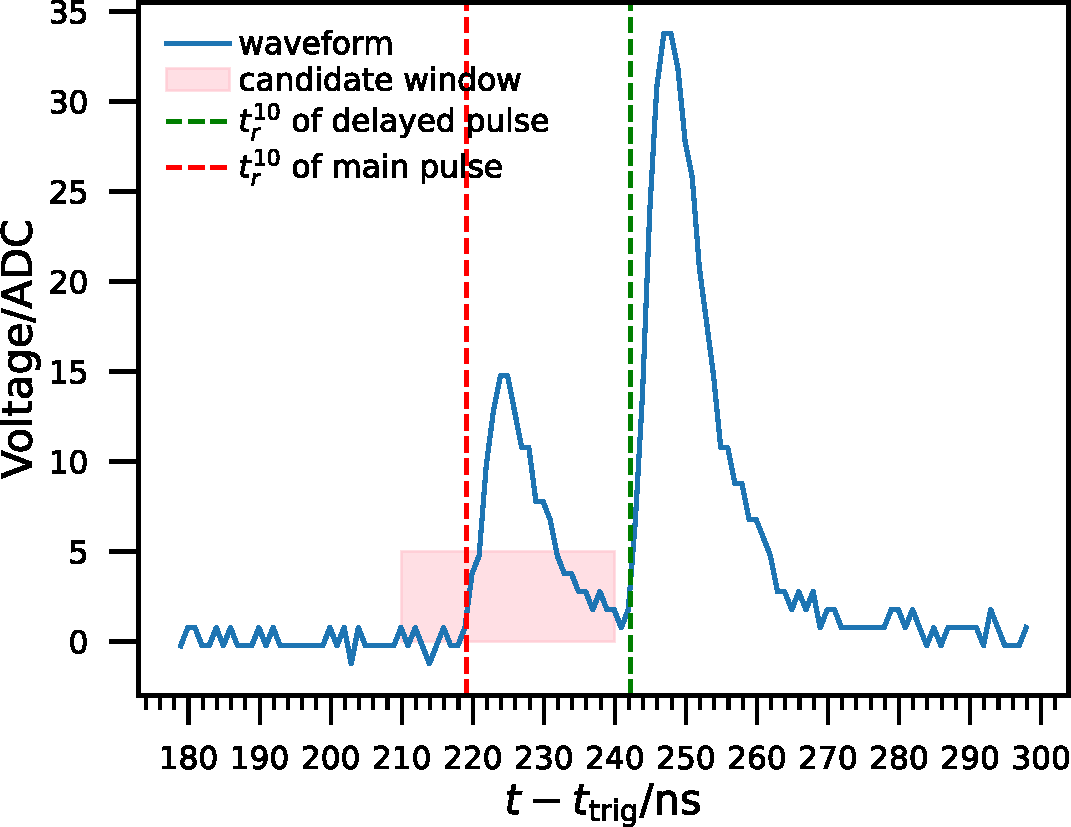
\includegraphics[width=\textwidth]{figures/method/triggerDoublePulse.pdf}
        \caption{}%PM
        \label{fig:triggerTT2pulse}
    \end{subfigure}
    \begin{subfigure}[t]{\SF\textwidth}
        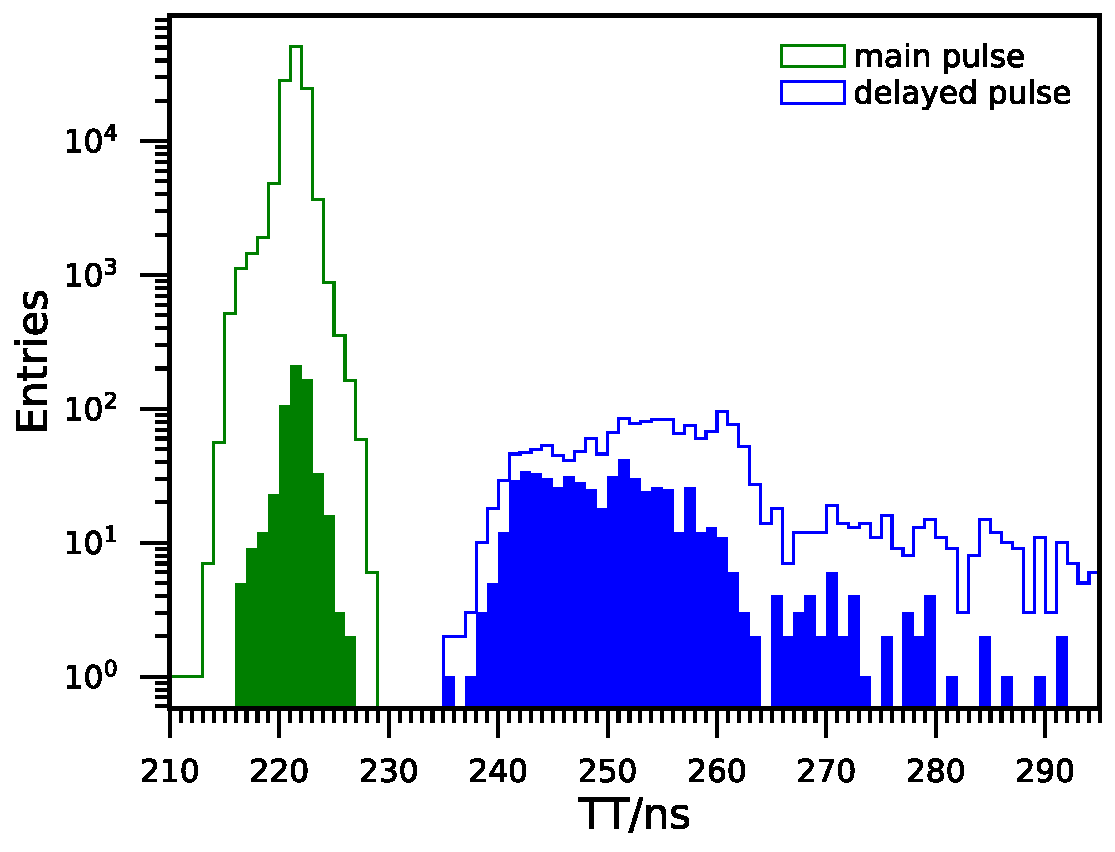
\includegraphics[width=\textwidth]{figures/method/triggerDelayedPulse.pdf}
        \caption{}%PM
        \label{fig:triggerTTlatepulse}
    \end{subfigure}
    \caption{(a) Double-pulse example. The first pulse falls in the candidate window defined in Section~\ref{sec:laserstage}. (b) The green and blue histograms are the main and delayed pulse distributions, respectively. The filled histograms are waveforms containing the main and delayed pulses simultaneously.}
\end{figure}

In Fig.~\ref{fig:triggerTTSLog}, the main and early components are modeled with Gaussian functions % padding
$N_1f_1^N(t;\mu_{\mathrm{TT}},\sigma_{\mathrm{TT}}^2)$ and $N_2f_2^N(t;\mu_K,\sigma_K^2)$, with the subscript $K$ standing for high-kinetic-energy PEs. Considering the exponential distribution of kinetic energies of secondary electrons~\cite{Furman,SecondElectron}, $f^\mathrm{Exp}(t;1/\tau_S)$ is suitable to model the delayed component.  We add a constant $b_S$ and a translation of $\mu_{TT} + 3\sigma_{TT}$ to fit the data. The \SI{0.5}{ns}-binned $\mathrm{TT}$ histogram with selection criteria in Section~\ref{sec:noisepeak} is fitted by

\begin{equation}
    \begin{aligned}
        B&+N_1f_1^N(t;\mu_{\mathrm{TT}},\sigma_{\mathrm{TT}}^2)\\
        &+N_2f_2^N(t;\mu_K,\sigma_K^2)\\
        &+b_SH(\mu_{\mathrm{TT}}+3\sigma_{\mathrm{TT}})+N_Sf^{\mathrm{Exp}}\left(t-(\mu_{\mathrm{TT}}+3\sigma_{\mathrm{TT}});\frac{1}{\tau_S}\right)
    \end{aligned}
\end{equation}
in which $H$ is the Heaviside function to restrict the domain of the delayed component, and $B$ is the constant dark noise rate. The early and exponential components are as small as $N_2/N_1 = \num{0.026\pm0.018}$, $N_S/N_1 = \num{0.010\pm0.003}$ and $2b_S\sigma_{\mathrm{TT}}/N_1 = \num{0.00026\pm0.00009}$ for the nine MCP-PMTs.  $\sigma_K$, $\tau_S$ and $\mu_{\mathrm{TT}}-\mu_K$ are fitted to be $\SI{1.4 \pm 0.3}{ns}$, $\SI{1.1\pm 0.1}{ns}$ and $\SI{3.0\pm 0.4}{ns}$. TTS ($\SI{1.73\pm0.08}{ns}$) is defined as FWHM$=2\sqrt{2\ln 2}\sigma_{\mathrm{TT}}$~\cite{HAMAMATSUManual} representing the timing resolution. The charge and TT seem to be correlated in Fig.~\ref{fig:triggerTTS2d} and the long tail is evident in charge distribution.

\begin{figure}[!htbp]
    \centering
    \begin{subfigure}[t]{\SF\textwidth}
        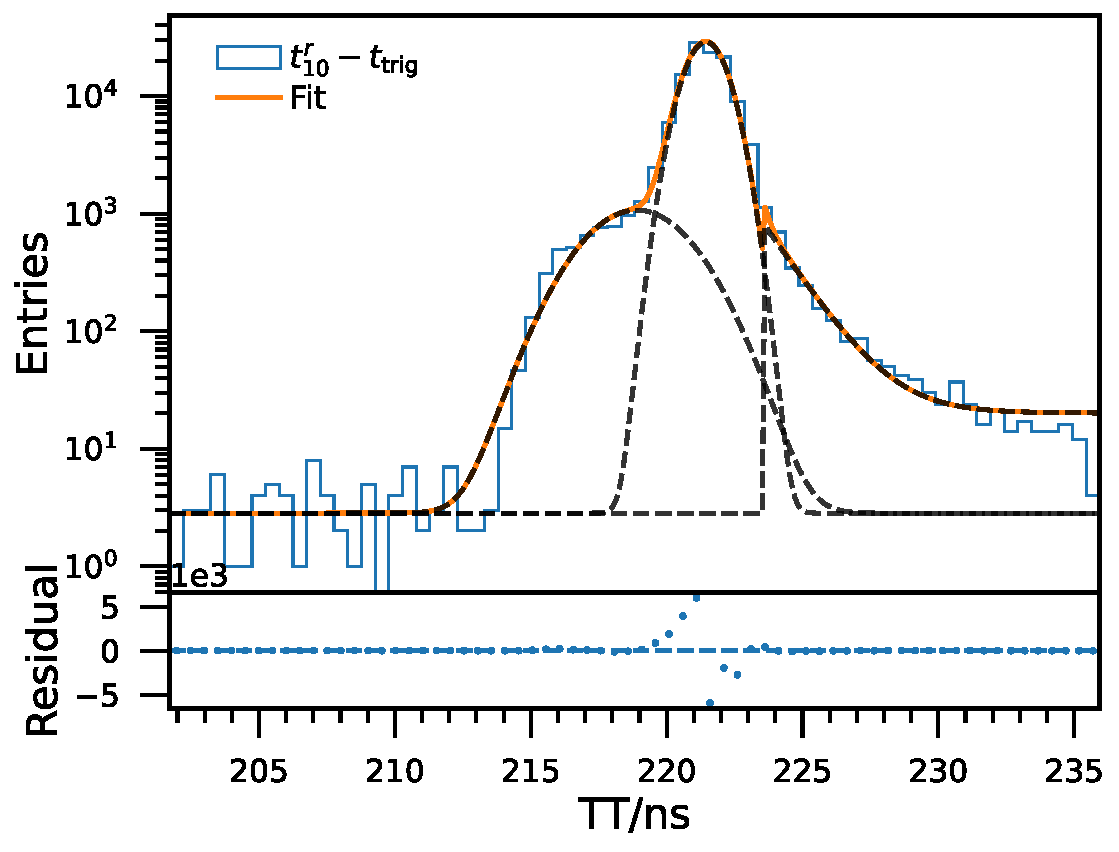
\includegraphics[width=\textwidth]{figures/method/triggerTTSLog.pdf}
        \caption{}%PM
        \label{fig:triggerTTSLog}
    \end{subfigure}
    \begin{subfigure}[t]{\SF\textwidth}
        \includegraphics[width=\textwidth]{figures/method/triggerTTS2d.pdf}
        \caption{}%PM
        \label{fig:triggerTTS2d}
    \end{subfigure}
    \caption{(a) The top pad is the distribution of TT with the y-axis in the logarithmic scale. The black dashed lines from left to right are early, main and delayed components with a dark noise pedestal. The bottom pad is the residual between data and fit in linear scale. (b) The 2D distribution of TT and charge with the colorbar in logarithmic scale.}
\end{figure}

\subsection{Dark count rate and pre-pulse}
\label{sec:dcr}
The dark noise mimicking PEs mainly comes from the spontaneous thermionic electrons emitted from the photocathode~\cite{KM3NetTesting}. The dark count rate (DCR) is ${N^{\mathrm{noise}}}/({N^{\mathrm{t}}T_{\mathrm{DCR}}})$, in which $N^{\mathrm{t}}$ is the number of total waveforms and $N^{\mathrm{noise}}$ is the noise count in the interval of $[\SI{-300}{ns},\SI{-150}{ns}]$ relative to the peak time $\mu_{\mathrm{TT}}$ of TT distribution with $T_{\mathrm{DCR}}=\SI{150}{ns}$. The DCR of nine MCP-PMTs is $5.8\pm\SI{1.6}{kHz}$ at room temperature.

Generated from photons hitting the MCP or the first dynode directly rather than the photocathode, \emph{pre-pulses} appear about tens of nanoseconds earlier with smaller amplitudes~\cite{JUNOMassTesting}. The probability $P_{\mathrm{pre}}$ of pre-pulses is $N^{\mathrm{pre}}/N^\mathrm{t} - \mathrm{DCR}\cdot T_{\mathrm{pre}}$, in which $N^{\mathrm{pre}}$ is the pre-pulse count of the total waveforms in the interval [\SI{-100}{ns},\SI{-10}{ns}] ($T_{\mathrm{pre}}=90$\,ns) relative to $\mu_{\mathrm{TT}}$. The small $P_{\mathrm{pre}}$ ($1\times10^{-6}\pm6\times10^{-6}$) is dominated by DCR at our low-occupancy setup.

\subsection{After-pulse}
\label{sec:afterpulse}
Ions such as \ce{H+}, \ce{He+} and \ce{O+} produced from gaseous impurities in the vacuum bulb by the PEs drift back to the photocathode, generate new electrons and then \emph{after-pulses}~\cite{JUNOMassTesting,Coates_1973}. The delay times of after-pulses are proportional to the square root of the mass-to-charge ratios of the ions~\cite{XENON1TTesting,Coates_1973,afterpulseTime}. %Considering electric field and $\frac{M}{Z}$ of ions, the travel time is in the scale of \si{us}.
\begin{figure}[!htbp]
    \centering
    \includegraphics[width=\LF\textwidth]{figures/method/triggerAfterpulseSchema.pdf}
    \caption{An example waveform for searching pre-pulses and after-pulses. Green and red vertical dashed lines are the trigger time and 10\% of the rising edge of the main pulse $t_r^{10}$, respectively. The gray and orange regions are the intervals for searching after-pulses and pre-pulses.}
    \label{fig:afterpulseSchema}
\end{figure}
The after-pulses are searched from \SI{200}{ns} after the main pulse in $N^\mathrm{hit}$ selected waveforms mentioned in Section~\ref{sec:noisepeak}. The 10\% rise time $t_r^{10}$ and charge $Q$ of the after-pulse and pre-pulse are calculated in the $[-\SI{10}{ns},\SI{75}{ns}]$ window relative to the peak position, as shown by the violet area in Fig.~\ref{fig:afterpulseSchema}.

The probability $P_{\mathrm{after}}$ of after-pulses is $N^{\mathrm{after}}/N^\mathrm{hit} - \mathrm{DCR}\cdot T_{\mathrm{after}}$, in which $N^{\mathrm{after}}$ is the pulse counts in [\SI{200}{ns}, \SI{9800}{ns}] ($T_{\mathrm{after}}=9600$\,ns) relative to the main pulses. $P_{\mathrm{after}}$ of nine MCP-PMTs is $0.009\pm0.005$.

\begin{figure}[!htbp]
    \centering
    \begin{subfigure}[t]{\LF\textwidth}
        \includegraphics[width=\textwidth]{figures/method/triggerAfterpulse1d.pdf}
        \caption{}%PM
        \label{fig:afterpulse1d}
    \end{subfigure}
    \begin{subfigure}[t]{\LF\textwidth}
        \includegraphics[width=\textwidth]{figures/method/triggerAfterpulse2d.pdf}
        \caption{}
        \label{fig:afterpulse2d}
    \end{subfigure}
    \caption{(a) An example of time distributions of dark noises (green), after-pulses (blue) and after-pulses with charge cut (orange) for an MCP-PMT, where the red line shows the Gaussian fits. The red point represents $N^{\mathrm{hit}}$ at \SI{0}{ns}, around which the pre-pulses and delayed pulses are not shown. The horizontal dash line illustrates the expected dark-noise level. (b) Charge versus time distribution of pre-pulses and after-pulses. The bright horizontal band at about 100\,$\mathrm{ADC}\cdot \mathrm{ns}$ mainly contains dark noise. The black (dash) line is the mean charge of (selected) pulses in each time bin.}
\end{figure}
% waveform analysis

The distribution of the delay time from $t_r^{10}$ of the main to after-pulse in Fig.~\ref{fig:afterpulse1d} indicates five structures at around \SI{300}{ns}, \SI{400}{ns}, \SI{600}{ns}, \SI{1200}{ns} and \SI{1700}{ns}, time ratio being about $1:\sqrt{2}:\sqrt{4}:\sqrt{16}:\sqrt{32}$. These structures may originate from \ce{H^+}, \ce{H_2^+}, \ce{He^{+}}, \ce{CH_4^+}, and \ce{N_2^+} or \ce{O_2^+}. XENON1T~\cite{XENON1TTesting} and XMASS~\cite{Abe_2020} gave the same assumptions for the first peak. But similar works by JUNO~\cite{Zhao:2022gks} and KM3NeT~\cite{KM3NetTesting} assigned the first peak to \ce{H_2^{+}}.

We use five Gaussians with DCR ($\sum_{i=1}^{5}{A_if_i^{\mathrm{AP}}(t;t_i,\sigma_i^2)} + \mathrm{DCR}\cdot N^{\mathrm{hit}}$) to model the five structures, in which $A_i$, $t_i$, and $\sigma_i$ are the amplitudes, times, width of each after-pulse structure (Table.~\ref{tab:afterpulse}). %The $A_i$s vary greatly for different MCP-PMTs.
A slow undulating structure contributes about half of the after-pulses on average in $[\SI{2000}{ns},\SI{7000}{ns}]$ as shown in Fig.~\ref{fig:afterpulse1d}, whose origin we are unable to identify.

\begin{table}
    \centering
    \caption{After-pulse parameters of MCP-PMTs}
    \label{tab:afterpulse}
    \begin{threeparttable}
        \begin{tabular}{c|ccccc}
            \hline\hline
            & \ce{H+} & \ce{H2+} & \ce{He+} & \ce{CH4+} & \ce{N2+} or \ce{O2+} \\
            \hline
            $t_i$/ns&300$\pm$4&414$\pm$25&596$\pm$53&1180$\pm$28&1714$\pm$29\\
            $A_i/N^{\mathrm{hit}}/10^{-3}$&1.6$\pm$1.1&0.5$\pm$0.3&0.2$\pm$0.2&1.1$\pm$0.7&1.9$\pm$0.6\\
            $\sigma_i$/ns&16$\pm$6&46$\pm$9 &33$\pm$10&44$\pm$11&70$\pm$20\\
            $Q_i/Q_0$&34$\pm$4&  -\tnote{*} &22$\pm$3&18$\pm$3&14$\pm$2\\
            $\sigma_{Q_i}/Q_0$&12$\pm$2&  -\tnote{*} &17$\pm$3&9$\pm$1&8$\pm$1\\
            \hline
        \end{tabular}
        \begin{tablenotes}
            \footnotesize
            \item[*] The charge of the 2nd structure cannot be fitted due to the interference with \ce{H+}.
        \end{tablenotes}
    \end{threeparttable}
\end{table}

% \begin{figure}[!htbp]
%     \centering
%     \begin{subfigure}[t]{\SF\textwidth}
%         \includegraphics[width=\textwidth]{figures/result/afterpulse.pdf}
%         \caption{}%PM
%         \label{fig:afterpulsePeak}
%     \end{subfigure}
%     \begin{subfigure}[t]{\SF\textwidth}
%         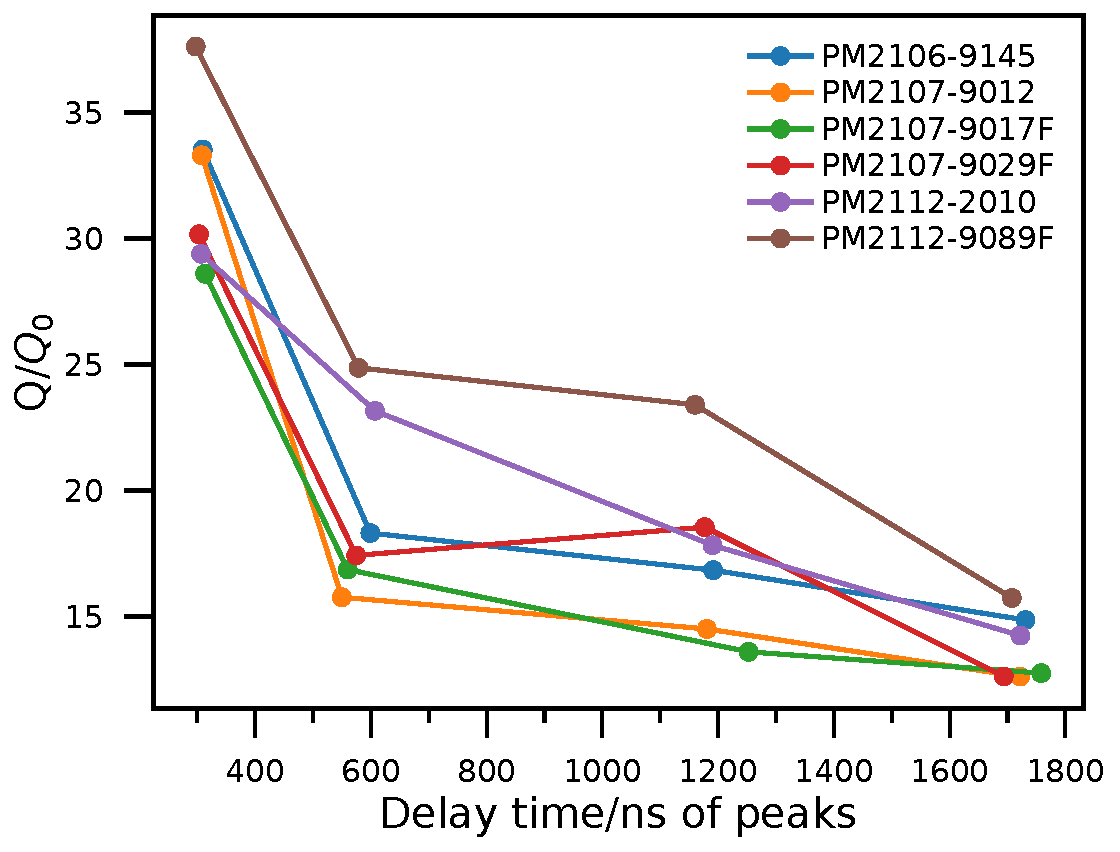
\includegraphics[width=\textwidth]{figures/result/afterpulseQ.pdf}
%         \caption{}%PM
%         \label{fig:afterpulseQ}
%     \end{subfigure}
%     \caption{(a) Time and relative amplitudes of after-pulse groups of 9 MCP-PMTs. (a) Time and mean charge of after-pulse groups of 6 MCP-PMTs.}
% \end{figure}

%The mean charge in each time bin shown as the black line. 
The after-pulses contain large charge signals, as shown in Fig.~\ref{fig:afterpulse2d}. The charge distributions in $[t_i-3\sigma_i,t_i+3\sigma_i]$ of each after-pulse are scaled to the same dark noise count in Fig.~\ref{fig:afterpulsecharge}.  Charge distribution of the second structure~(\ce{H2+}) is hard to fit due to the interference with the first one~(\ce{H+}).  We fit each charge distribution with a Gaussian $f^{\rm APQ}_i(Q;Q_i,\sigma_{Q_i}^2)$, in which $Q_i$ and $\sigma_{Q_i}$ are the charge and spread of each after-pulse (Table.~\ref{tab:afterpulse}). Because the 3rd-structure charge distribution is dominated by charge less than 700\,ADC$\cdot$ns as shown in Fig.~\ref{fig:afterpulse2d} and Fig.~\ref{fig:afterpulsecharge}, $\sigma_{Q_3}$ from fitting on low-statistic entries contains large uncertainty and maybe unreliable. From the six PMTs with higher occupancies, the mean charge of each after-pulse shows a negative correlation between charge and delay time.

\begin{figure}[!htbp]
    \centering
    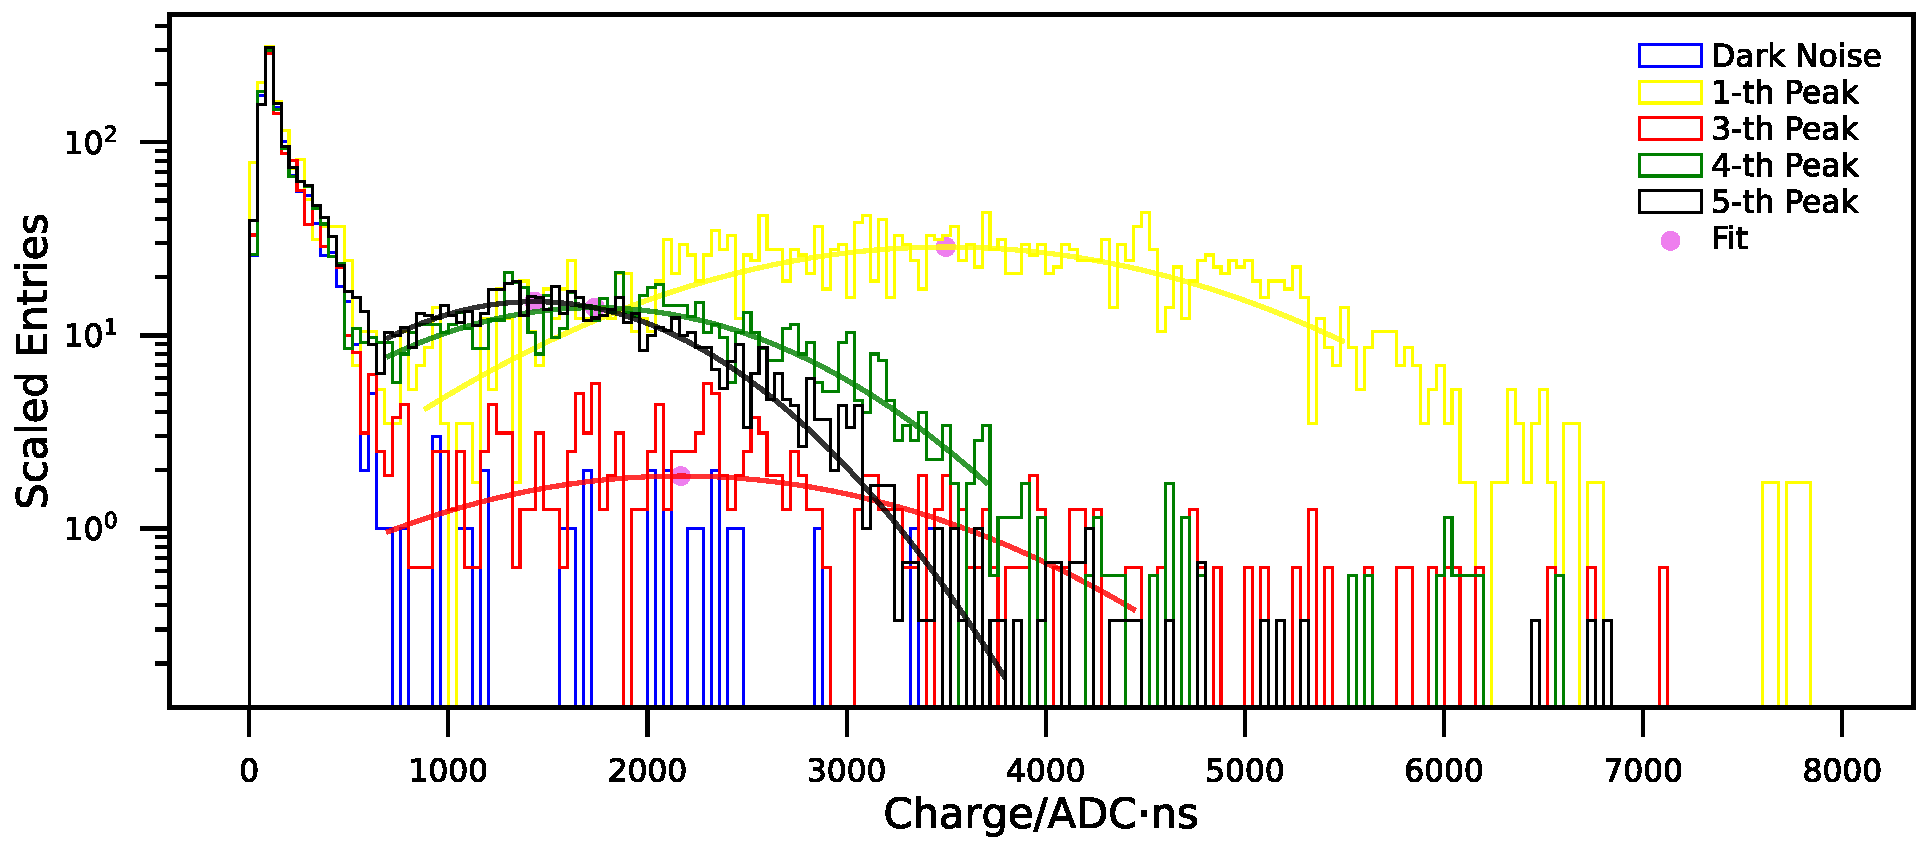
\includegraphics[width=\textwidth]{figures/method/triggerafterpulseCharge.pdf}
    \caption{The charge distribution of after-pulse structures of an example MCP-PMT. The blue histogram is the distribution of dark noise. The violet points are the peaks of fit curves.}
    \label{fig:afterpulsecharge}
\end{figure}

\subsection{Relative photon detection efficiency}
\label{sec:PDE}
 %For example, JUNO fixed one reference PMT to calibrate the light intensity and other reference PMTs are circulated through all channels to calibrate the light allocation ratio~\cite{Wonsak_2021}.
A regression method is developed to combine the light-source calibration and PDE measurements simultaneously. Let $I_n$ denote the light intensity of the $n$th run, $\alpha_j$ the light allocation ratio of the $j$th splitter channel (out of four and assumed to be stable across runs), and $\epsilon_k$ the PDE of the $k$th PMT (out of one reference dynode and nine MCP-PMTs). The PE counts in each waveform follow Poisson distribution $\pi(I_n\alpha_j\epsilon_k)$.

For convenience, the index of the reference PMT is set to 0. Let $\alpha_j^0\equiv\alpha_j/{\alpha_0}$, $\epsilon_k^0\equiv\epsilon_k/{\epsilon_0}$, $I_n^0\equiv I_n\alpha_0\epsilon_0$.  The hit rate $R_{njk}$ of the $k$th PMT at the $j$th channel in the $n$th run is

\begin{equation}
    \label{equ:linkfunction}
    R_{njk}=1-\exp\left(-I_n\alpha_j\epsilon_k\right)=1-\exp\left(-e^{\log{I_n^0}+\log{\alpha_j^0}+\log{\epsilon_k^0}}\right).
\end{equation}

The number of hit waveforms $N^{\mathrm{hit}}_{njk}$ of the $k$th PMT in the $n$th run with the $j$th channel follows Binomial distribution $B(N^{\mathrm{hit}}_{njk};R_{njk},N^t_{njk})$, in which $N^t_{njk}$ is the total number of waveforms by the laser trigger. The likelihood is therefore

\begin{equation}
    \label{equ:likelihood}
    \mathcal{L}=\prod_{njk}{R_{njk}^{N^\mathrm{hit}_{njk}}(1-R_{njk})^{N^t_{njk}-N^{\mathrm{hit}}_{njk}}}.
\end{equation}

Eqs.~\eqref{equ:linkfunction} and \eqref{equ:likelihood} define a \emph{Binomial regression} with \emph{complementary log-log} link function~\cite{glm}, with $\log{\epsilon_k^0}$, $\log{\alpha_j^0}$ and $\log{I_n^0}$ as parameters. The relative PDEs $\epsilon_k^0$ of MCP-PMTs are calculated from the regression results to be about $1.71$, significantly higher than the reference PMT.  We could attribute it to the improvements on both quantum and collection efficiencies of the GDB-6082 MCP-PMTs.
